\section{Regulering}\label{sec:regulering}

Som vist i afsnit xx, er det omvendte pendul et grundlæggende ustabilt system.
I ligning xx blev overførelses funktionen for pendulet fysiske system fundet.
Hvis der ses bort fra de udefra kommende forstyrrelser, vil pendulets overførelses funktion være.
\begin{align}
H_{pendul}(s) = \frac{1}{Ls^2 - g} \label{eq:h_pendul}
\end{align} 
Dette system har 2 reelle poler liggende i $s = \pm\sqrt{g/L}$.
Her ses det at systemet har en pol liggende på den positive s-akse, i $s = \sqrt{g/L}$, som giver systemet sin ustabilitet.

Ved at anvende klassisk reguleringsteori, kan der ud fra systemets openloop overførelsesfunktion $H_{OL}$ findes frem til, hvilken regulator der skal til for at give et stabilt system, når reguleringssystemet lukkes.   

\subsection{Bestemmelse af Openloop for hele systemet}
For at kunne beskrive en openloop overførelsesfunktion for hele systemet er vi nød til at samle op på følgende.
Overførelsesfunktioner for Pendul, Motor, Vogn, Filter, Ensretter og signal summation.
\begin{figure}[h!]
	\centering
	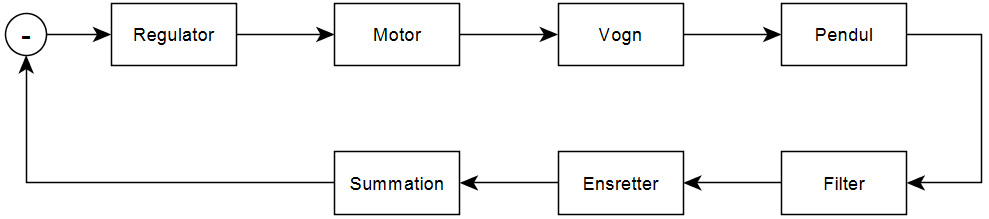
\includegraphics[width=.8\textwidth]{billeder/reg_diagram.png}
	\caption{Diagram over alle overførelsesfunktions-blokke i systemet.}
	\label{fig:reg_diagram}
\end{figure}
\FloatBlock 

I figur \ref{fig:reg_diagram} fremgår alle overførelsesfunktioner i hele systemet som skal beskrives.
De enkelte blokke vil her blive opsummeret og gennemgået, startende fra summations punktet i figur \ref{fig:reg_diagram}.

Regulatoren der er det endelige mål, indgår ikke i $H_{ol}$ og bliver derfor sat til $H_{reg} = 1$.   

Motorens dynamik beskrevet i afsnit \ref{sec:sec_motorstyring}, ligning \ref{eq:motor_trans} giver os den elektriske dynamik for motoren
\begin{align}
H_{motor}(s) = \frac{\num{18E-3}s}{\num{18E-3}s +1}
\end{align}

For at kunne beskrive selv vognen, blev der i afsnit \ref{sec:sec_motoroverforelse} udledt ligning \ref{eq:vogn_dynamic_trans}
\begin{align}
H_{vogn}(s) =\frac{0,66}{s} + \frac{1,37}{s^2} 
\end{align}
Under målingerne af vognens dynamik i afsnit \ref{sec:sec_motoroverforelse} kom det frem, at der skulle en hvis strømstyrke til for at få vognen i bevægelse.
Vi vælger derfor kun at medtage den del at dynamikken der ligger inde for det område hvor vognen er i bevægelse og ser derfor bort fra, at vi ikke kan beskrive den dynamik der ligger mellem $-1 \si{\ampere} < I < 1 \si{\ampere}$. 
Således kan dynamikken for vognen forenkles til
\begin{align}
 H_{vogn}(s) = \frac{1,37}{s^2} 
\end{align}

For pendulet vil vi anvende $H_{pendul}$ i ligning \ref{eq:h_pendul}.
\begin{align}
H_{pendul}(s) = \frac{1}{Ls^2 - g} 
\end{align}

I afsnit \ref{sec:filter} bliver indgangsfilteret dimensioneret med en resonansfrekvens på $f_0 = 44,557 \si{\kilo\hertz}$, og en forstærkning på $h_0 = 3,5$. 
Selv om indgangsfilteret er designet som et båndpas-filter, vil vi i reguleringen anse det som et lavpas-filter.
Således vil overførelsesfunktionen for filteret kunne forenkles til 
\begin{align}
H_{filter}(s) = \frac{H_0}{(2 \pi f_0)^{-1}s +1} = \frac{3,5}{\num{3.571E-06}s +1}
\end{align}

Ligeledes kan den designede ensretning af feedback signalet efter filteret, beskrives som et lavpas-filter.
Den beregnede tidskonstant $\tau = 470 \si{\micro\second}$ angiver tidskonstanten i dynamikken for ensretningen og kan beskrives som
\begin{align}
H_{ensretter}(s) = \frac{1}{\tau s +1} = \frac{1}{\num{4.70E-4}s +1}
\end{align} 

Endeligt samles de to indkommende signaler fra sensor spolerne i et summationspunkt, beskrevet i afsnit \ref{sec:summa}.
Her er dynamikken i den anvendte instrumenteringsforstærker udeladt og kun signalforstærkningen er medtaget.
\begin{align}
H_{summa}(s) = 4,5
\end{align}  

\subsection{Forhold mellem sensor signal og pendul vinkel}
Det er i dimensioneringen af vores reguleringssystem, vigtigt at kende forholdet mellem pendulets vinken $\theta$ og signalstyrken på indgangen til filteret.
\husk{JJ}{theta indgangssignal måling og kommentar at den ikke kan bruges}


\subsection{Dimensionering og valg af regulator}
Ud fra xx, ses det at en forøgelse af fasemarginen ved xx rad/s, vi kunne give et stabilt system.
\husk{JJ}{Beskrivelse fra matlab beregninger og Reg bog}


\subsection{Simulering af reguleret system}
\begin{figure}[h!]
	\centering
	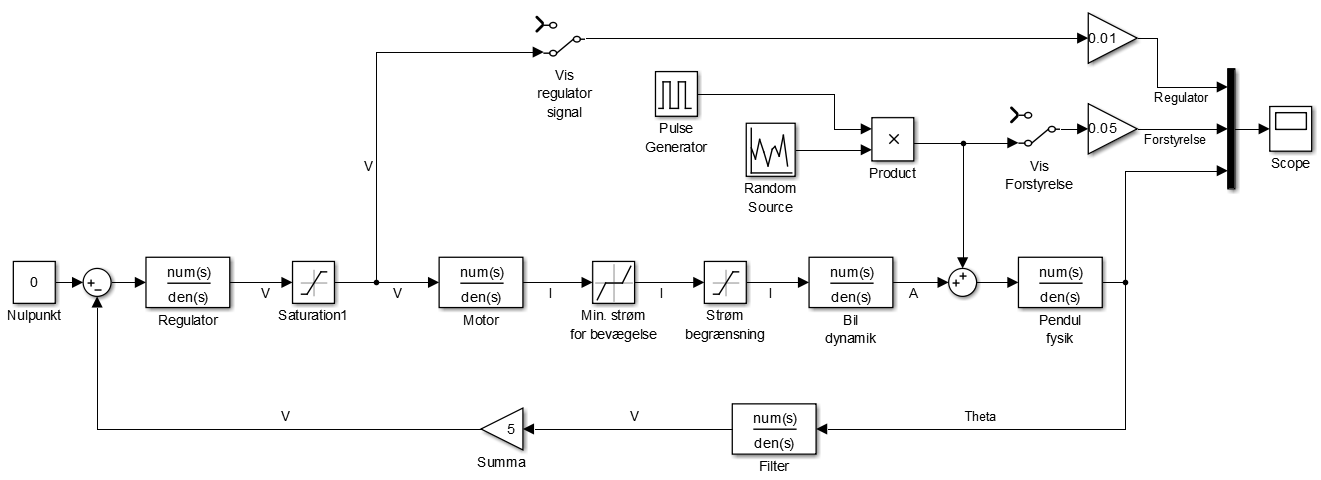
\includegraphics[width=1\textwidth]{billeder/transfunc_sim.png}
	\caption{Simulink simulering model af det samlede system.}
	\label{fig:transfunc_sim}
\end{figure}
\FloatBlock 


\begin{figure}[h!]
	\centering
	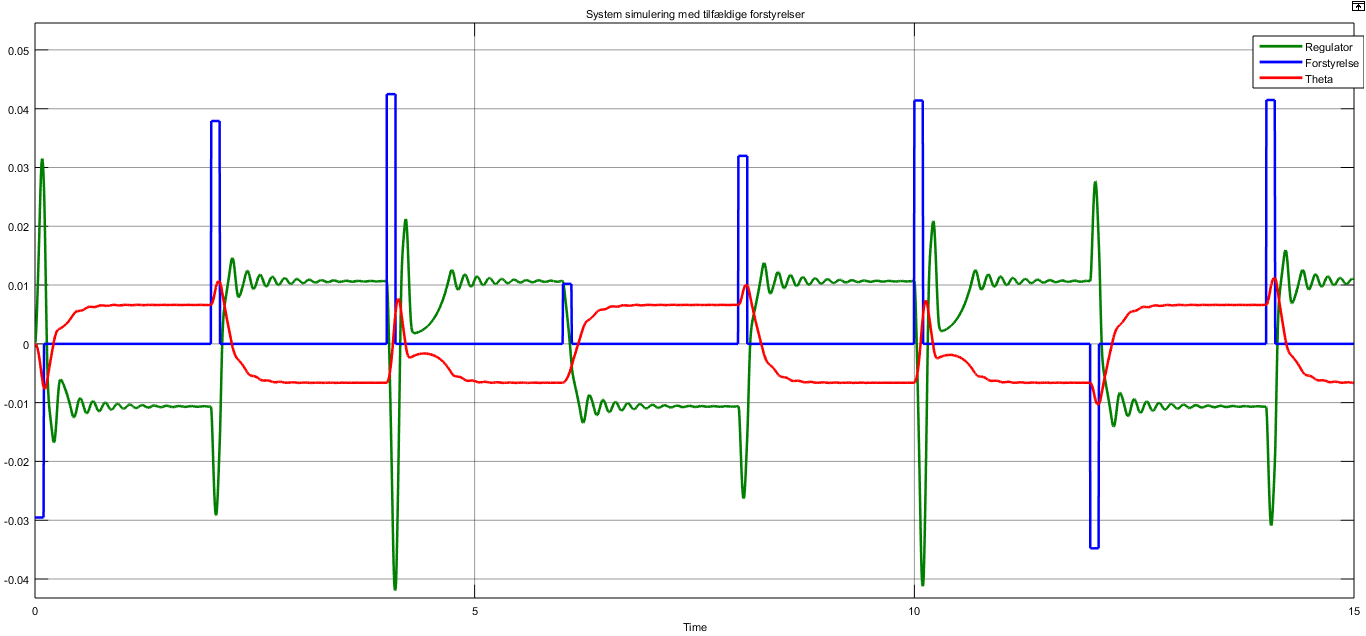
\includegraphics[width=1\textwidth]{billeder/system_sim_stimuli.png}
	\caption{Systemsimulering med tilfældige forstyrrelser.}
	\label{fig:system_sim_stimuli}
\end{figure}
\FloatBlock 

\husk{JJ}{kort beskrivelse af simulering og resultat}

\subsection{Implementering af regulator}
\begin{figure}[h!]
\centering
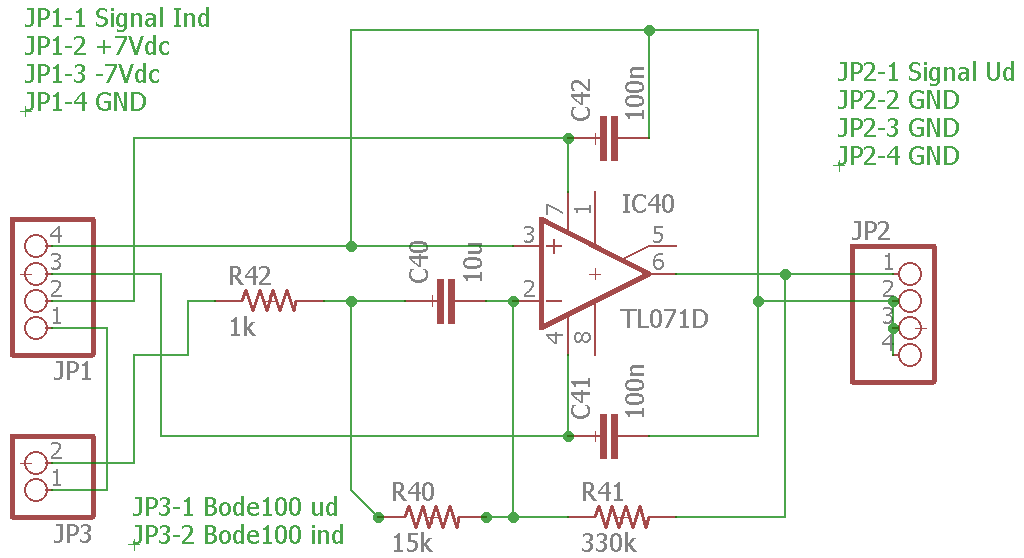
\includegraphics[width=.8\textwidth]{billeder/pd_schematic.png}
\caption{Kredsløbsdiagram af den implementerede PD regulator.}
\label{fig:pd_schematic}
\end{figure}
\FloatBlock 

\husk{JJ}{Udledning af komponent størrelser}


\section{Delkonklusion af regulering og motorstyring}
\husk{JJ}{Samle op her}







%\begin{itemize}
%	\item Valg af regulator-type (PD)
%	\item Evt. måling af loop gain 
%	\item Saturation punkter
%	\item Stabilitet
%\end{itemize}



